\input{./econtexRoot.texinput}
\documentclass[pdflatex]{beamer}
\usepackage{\LaTeXInputs/EGMN-Slides}

\newbool{buffstk}\global\booltrue{buffstk}%\boolfalse{buffstk}
\newbool{bristol}\global\booltrue{bristol}%\boolfalse{bristol}
\newbool{bundesb}\global\booltrue{bundesb}\boolfalse{bundesb}
\usepackage{\econark,\econtexShortcuts}

% _____________ Opening slide _______________________

\ifbool{buffstk}{% For bufferstock paper
  \title[Buffer Stock Theory]{Theoretical Foundations of Buffer Stock Saving}
  \author[Carroll]{Chris Carroll}
  \institute[JHU]{Johns Hopkins University}
  \date[\today]{September 12, 2019  \\ \medskip \medskip \medskip \href{https://econ-ark.org/}{\small Powered By} \\ 
\includegraphics[width=0.5in]{\econtexRoot/Resources/econ-ark-logo-small.png}}
}{}


\title[Stimulus]{Welfare and Spending Effects of Consumption Stimulus Policies}
\author{
  Christopher D. Carroll
  \and
  Edmund Crawley
}

\ifbool{bristol}{% set date for bristol presentation
  \date[\today]{September 12, 2019  \\ \medskip \medskip \medskip \href{https://econ-ark.org/}{\small Powered By} \\ 
\includegraphics[width=0.5in]{\econtexRoot/Resources/econ-ark-logo-small.png}}
}{}

\ifbool{bundesb}{% set date for bundesbank
  \date[\today]{September 12, 2019  \\ \medskip \medskip \medskip \href{https://econ-ark.org/}{\small Powered By} \\ 
\includegraphics[width=0.5in]{\econtexRoot/Resources/econ-ark-logo-small.png}}
}{}


\begin{document}\bibliographystyle{\econtexBibStyle}

\begin{frame}[plain]
    \titlepage
\end{frame}


% _____________ 1st section  ____________

\ifbool{buffstk}{
    \section{Introduction}
    \subsection{Motivation}

    \begin{frame}
        \frametitle{Drawbacks of Numerical Solutions}


        \pause A Black Box \pause
        \begin{itemize}
            \item Can Construct Solution to Model Without Really Understanding It
            \item Hard Even To Be Sure Your Numerical Solution Is {\it Right}
            \item Little Intuition for How Results Might Change With
                  \begin{itemize}
                      \item Calibration
                      \item Structure
                  \end{itemize}
            \item {\it Very} Hard To Teach!
        \end{itemize}

        \medskip\medskip
        \pause I Am A {\it Big} Fan Of Numerical Methods
        \begin{itemize}
            \item Have Done A Good Deal Of Work With Them Myself
            \item But As A Result, Have Felt All These Drawbacks Keenly
        \end{itemize}



    \end{frame}


}{}


\subsection{Lorenz}
\begin{frame}
    \frametitle{The Lorenz Figure}
    \centerline{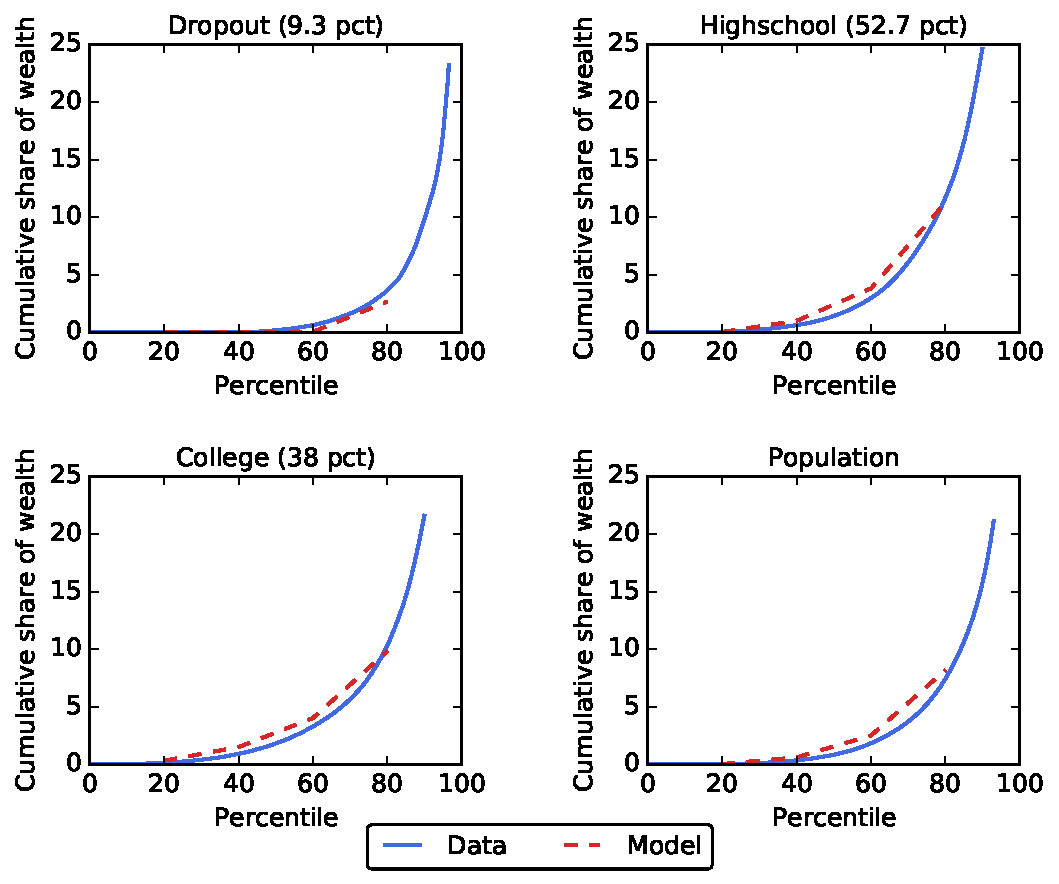
\includegraphics[width=4in]{\FigDir/LorenzPoints.pdf}}
\end{frame}

\end{document}

